\chapter{RESULTADOS\label{sec:resultados}}

\clearpage

Este capítulo analiza los resultados de las pruebas no funcionales centradas en el rendimiento de la aplicación web de mensajería instantánea desarrollada en el capítulo anterior. Para, posteriormente, justificar si la solución web propuesta en este documento cumple con los requisitos mínimos de integración en las aplicaciones de emergencias para teléfonos móviles.

Seguimos con la metodología de pruebas de rendimiento según Microsoft Developer Network. Ya hemos ejecutado y monitorizado las pruebas. Hemos recogido los resultados y vamos con el último paso.

\section{Analizar los resultados y realizar un informe}

En la última fase, se consolida y comparte los resultados de la prueba. Analizamos los datos, tanto individualmente como con un equipo multidisciplinario. Volvemos a priorizar el resto de las pruebas y a ejecutarlas en caso de que sea necesario.

Cuando todas las métricas estén dentro de los límites aceptados, ninguno de los umbrales establecidos hayan sido rebasados y toda la información deseada se ha reunido, las pruebas han acabado para el escenario definido por la configuración \cite{jmeter6}.

Ahora que tenemos los resultados, vamos a destacar tres casos.

\subsection{Prueba de 300 salas, 10 usuarios por sala y 1 mensaje cada 2,5 segundos}

El primer caso es el caso más extremo que podría darse en un centro 112, ya que tendríamos todos los operadores (300) usando el servicio de IM, al mismo tiempo que también personal de soporte (digamos que 10 usuarios por sala) y enviando mensajes con una frecuencia real (1 mensaje cada 2,5 segundos).

\begin{figure}[htp!]
  \centering
  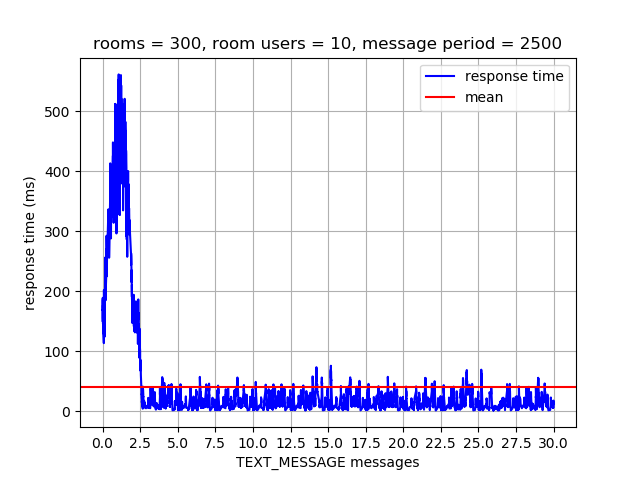
\includegraphics[scale=0.6,clip=true]{chat_r300_u10_m2500}
  \caption{Prueba de 300 rooms, 10 room users y 2500 msg period}
  \label{fig:chat_r300_u10_m2500}
\end{figure}

Como podemos observar en la gráfica, al principio el tiempo de respuesta es peor ya que el sistema se prepara y luego reutiliza recursos por lo que el resto de mensajes ya tienen un tiempo más similar.

Algunos valores a destacar son:

\begin{itemize}
  \item \textbf{Media}: 40.5384253862 ms
  \item \textbf{Desviación típica}: 81.8405749338 ms
  \item \textbf{Varianza}: 6697.87970549 ms
  \item \textbf{Mensajes por segundo}: 152.561093902 msg/s
\end{itemize}

\subsection{Prueba de 300 salas, 20 usuarios por sala y 1 mensaje cada segundo}

En el segundo caso se ha tenido en cuenta que el personal del centro 112 no ha incrementado (300 salas), pero el número por sala al llegado al máximo permitido (20 usuarios por sala) y la frecuencia de envío de mensajes a incrementado (1 mensaje por segundo).

\begin{figure}[htp!]
  \centering
  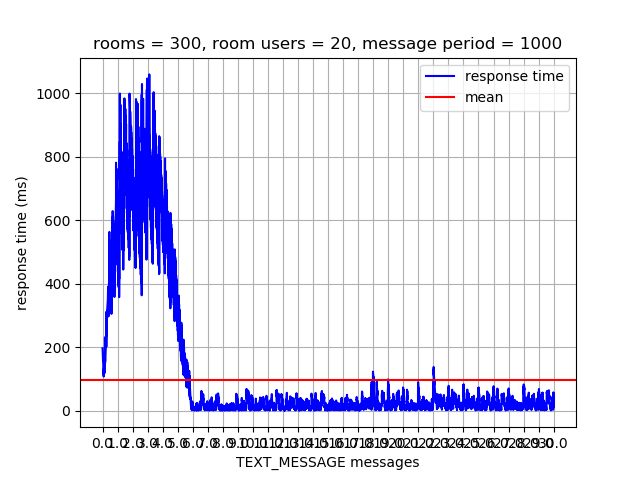
\includegraphics[scale=0.6,clip=true]{chat_r300_u20_m1000}
  \caption{Prueba de 300 rooms, 20 room users y 1000 msg period}
  \label{fig:chat_r300_u20_m100}
\end{figure}

Como podemos observar en la gráfica, al principio el tiempo de respuesta es mucho peor que el primer caso. El sistema tarda más tiempo en prepararse ya que son más usuarios enviando mensajes y conexiones WebSocket que mantener.

Algunos valores a destacar son:

\begin{itemize}
  \item \textbf{Media}: 97.3029789368 ms
  \item \textbf{Desviación típica}: 202.136129895 ms
  \item \textbf{Varianza}: 40859.015009 ms
  \item \textbf{Mensajes por segundo}: 373.925825854 msg/s
\end{itemize}

\subsection{Prueba de 400 salas, 20 usuarios por sala y 1 mensaje cada segundo}

En el último caso, a diferencia del anterior, se ha incrementado también el número de salas (400).

\begin{figure}[htp!]
  \centering
  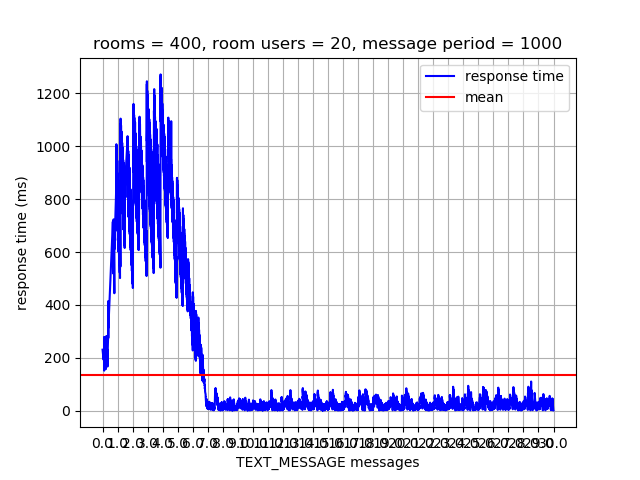
\includegraphics[scale=0.6,clip=true]{chat_r400_u20_m1000}
  \caption{Prueba de 400 rooms, 20 room users y 1000 msg period}
  \label{fig:chat_r400_u20_m1000}
\end{figure}

Como podemos observar en la gráfica, al principio el tiempo de respuesta es mucho peor que el segundo caso como era de esperar. Pero luego también consigue estabilizarse y dar buenos resultados.

Algunos valores a destacar son:

\begin{itemize}
  \item \textbf{Media}: 136.955281374 ms
  \item \textbf{Desviación típica}: 266.528534589 ms
  \item \textbf{Varianza}: 71037.4597502 ms
  \item \textbf{Mensajes por segundo}: 339.918519629 msg/s
\end{itemize}
